\documentclass[14pt]{beamer}
\usepackage[T2A]{fontenc}
\usepackage[utf8]{inputenc}
\usepackage[english,russian]{babel}
\usepackage{amssymb,amsfonts,amsmath,mathtext}
\usepackage{cite,enumerate,float,indentfirst}
\usepackage{booktabs}

\graphicspath{{images/}}

\usetheme{Pittsburgh}
\usecolortheme{whale}

\setbeamercolor{footline}{fg=blue}
\setbeamertemplate{footline}{
  \leavevmode%
  \hbox{%
  \begin{beamercolorbox}[wd=.333333\paperwidth,ht=2.25ex,dp=1ex,center]{}%
    Куликов А.В., ABBYY-MIPT
  \end{beamercolorbox}%
  \begin{beamercolorbox}[wd=.333333\paperwidth,ht=2.25ex,dp=1ex,center]{}%
    Москва, 2016
  \end{beamercolorbox}%
  \begin{beamercolorbox}[wd=.333333\paperwidth,ht=2.25ex,dp=1ex,right]{}%
  Стр. \insertframenumber{} из \inserttotalframenumber \hspace*{2ex}
  \end{beamercolorbox}}%
  \vskip0pt%
}

\newcommand{\itemi}{\item[\checkmark]}

\title{\small{Японский: буквенные n-граммы для распознавания}}
\subtitle{\footnotesize{Контроль НИР}}
\author{\small{%
~Куликов А.В., гр. 397\\%
\emph{Руководитель:}~Андрианов А.И.}\\%
\vspace{30pt}%
ABBYY-MIPT%
\vspace{20pt}%
}
\date{\small{Москва, 2016}}

\begin{document}

\maketitle

\begin{frame}

\frametitle{Задача}
\begin{itemize}
    \item Japanese kanji/kana OCR.
    \item Существуют путающиеся символы, например:
    \begin{figure}[h]
        \center{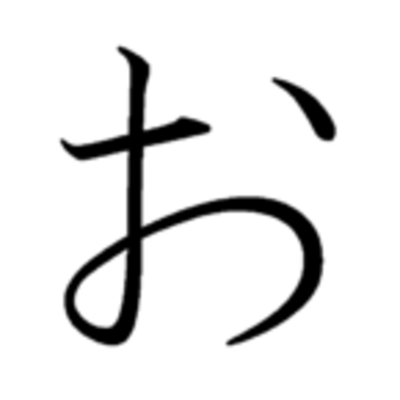
\includegraphics[scale=0.05]{KanaO}\ и 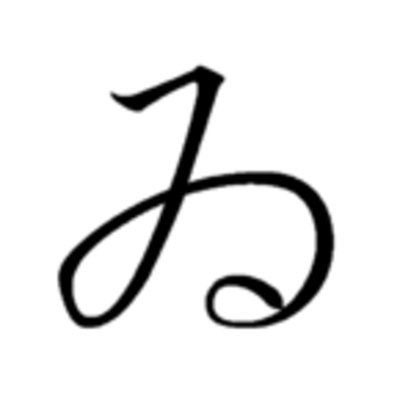
\includegraphics[scale=0.05]{KanaWi}}
    \end{figure}
    \item \emph{Цель работы: } построить и сравнить различные эвристики для исправления ошибок OCR, используя буквенную n-граммную модель японского языка.
\end{itemize}
\end{frame}

\begin{frame}
\frametitle{Текущие результаты}
\begin{itemize}
    \item Был выбран, получен и адаптирован корпус;
    \item Были получены статистики по n-граммам;
    \item Был разработан настраиваемый алгоритм для зашумления корпуса;
    \item Был определён Baseline;
    \item Были получены первые результаты.
\end{itemize}
\end{frame}

\begin{frame}
\frametitle{Корпус}
\begin{itemize}
    \item Корпус html-страниц с различных сайтов, доступный компании ABBYY;
    \item Был приведён к plain-utf-8 представлению;
    \item Итоговый размер $\approx 1.5$ GB;
    \item Был разделён на 3 неравных подкорпуса (debug/train/test).
\end{itemize}
\end{frame}

\begin{frame}
\frametitle{Корпус -- исходные кодировки}
\begin{center}
\begin{tabular}{ll}
Документов & Кодировка \\
68789 & utf-8 \\
46870 & iso-8859-2 \\
42015 & shift\_jis \\
2562 & euc-jp \\
1575 & cp932 \\
544 & ascii \\
436 & windows-1253 \\
256 & iso-8859-7 \\
$\approx 5\%$ & ещё 6 штук \\
\end{tabular}
\end{center}
\center{ Всего около 160k документов.}
\end{frame}

\begin{frame}
\frametitle{Корпус -- статистики по n-граммам}
\begin{itemize}
  \item Получены по train-подкорпусу ($\approx 400MB$):
\end{itemize}
\begin{center}
\begin{tabular}{lllll}
n & bins & outcomes & size ($\approx$) & time ($\approx$) \\
1-gram & 5188 & 2283229 & 100 KB & 2 mins \\
2-gram & 402035 & 5426594 & 6.8 MB & 50 mins \\
3-gram & 2455307 & 10407170 & 48.7 MB & 2 hrs
\end{tabular}
\end{center}
\begin{itemize}
  \item Сериализованы в pickle-dump nltk.FreqDist (весьма эффективно по памяти).
\end{itemize}
\end{frame}

%\begin{frame}
%\frametitle{Корпус -- статистики по n-граммам}
% Картинку?
%\end{frame}

\begin{frame}
\frametitle{Пошумим}
\begin{itemize}
    \item Список частых OCR-ошибок:
\end{itemize}
    \center{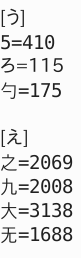
\includegraphics[scale=0.5]{1.png}}
\begin{itemize}
    \item Различные стратегии замены (абсолютное/относительное значение, какой символ подставлять и т.д.).
\end{itemize}
\end{frame}

\begin{frame}
\frametitle{Скоринг текста}
\begin{itemize}
    \item Текст бьётся на предложения (по пробельным символам и знакам препинания);
    \item Оценка предложения -- среднее геометрическое частот его n-грамм (больше-лучше);
    \item Если максимальную оценку получил этанол -- хорошо;
    \item Оценка текста -- процент предложений, где лидирует эталон.
\end{itemize}
\end{frame}

\begin{frame}
\frametitle{Baseline}
\begin{itemize}
    \item Оценка текста по униграммной модели;
    \item Да, по одиночным символам;
    \item Зато такой Baseline легко побить!
\end{itemize}
\end{frame}

\begin{frame}
\frametitle{Результаты -- 1}
\begin{itemize}
  \item Замена 1 любого символа в предложении на самый частый:
\end{itemize}
\begin{center}
\begin{tabular}{ll}
n & mean percentage \\
1-gram & 51.688 \% \\
2-gram & 89.256 \% \\
3-gram & 88.681 \%
\end{tabular}
\end{center}
\end{frame}

\begin{frame}
\frametitle{Результаты -- 2}
\begin{itemize}
  \item Замена 1 любого символа в предложении на случайный из возможных:
\end{itemize}
\begin{center}
\begin{tabular}{ll}
n & mean percentage \\
1-gram & 48.989 \% \\
2-gram & 83.741 \% \\
3-gram & 87.363 \%
\end{tabular}
\end{center}
\end{frame}

\begin{frame}
\frametitle{Что делать дальше?}
\begin{itemize}
  \item Экспериментировать с паттернами шума на корпусе и скорингом;
  \item Умный back-off для n-грамм при оценивании;
  \item Попробовать учитывать грамматические хвосты и варианты словного деления;
  \item Выкинуть хвосты распределения символов для оптимизации.
\end{itemize}
\end{frame}

\begin{frame}
\frametitle{Список литературы}
\footnotesize{
\begin{itemize}
  \item Foundations of Statistical Natural Language Processing / \\C. D. Manning, H. Schutze.
  \item Efficient In-memory Data Structures for N-Grams Indexing / \\D. Robenek, J. Platos, V. Snasel
  \item Applying Conditional Random Fields to Japanese Morphological Analysis / T. Kudo, K. Yamamoto, Y. Matsumoto
\end{itemize}}
\end{frame}

%%%%%%%%%%%%%%%%%%%%%%%%%%%%%%

\begin{frame}
\center{\huge
Спасибо
}
\end{frame}

\end{document} 